\chapter{Estado del Arte}\label{chapter:state-of-the-art}

El laboratorio de tecnolog\'ia RF y comunicaciones m\'oviles de la Universidad de Ciencias Aplicadas de Osnabrück en Alemania en noviembre del 2020 realiz\'o un estudio al rendimiento de la plataforma de Hyperledger Fabric en su versi\'on 2.0, estrenada en febrero de ese mismo a\~no [\cite{dreyer2020performance}].

El prop\'osito de ese trabajo fue obtener una evaluaci\'on definitiva de c\'omo la escala de los diferentes participantes de la red influyen en el rendimiento de la red de Fabric. En particular, el n\'umero de pares, organizaciones, nodos ordenadores y tama\~no de bloque. Desarrollaron su propia herramienta [\cite{Configurator}] para Fabric 2.0 que generar autom\'aticamente la red requerida que contiene el n\'umero deseado de componentes e instala el contrato inteligente de prueba autom\'aticamente. Las m\'etricas de rendimiento no se miden directamente. Emplearon las siguientes f\'ormulas para obtenerlas:\\

\emph{Rendimiento} $ = \frac{1s}{\frac{ \sum_i^N t\_tx_i } {N} }$ [TPS]\\

\emph{Tasa de Error} $ = \frac{F}{N} \cdot 100\% $\\


\emph{Latencia} $ = t\_tx_i + t\_b_i$ [ms]

{\vspace{1 cm}}

donde:
\begin{itemize}
\item $t\_tx_i$ es el tiempo de la i-\'esima transacci\'on.
\item $t\_b_i$ es el tiempo de confirmaci\'on del i-\'esimo bloque.
\item $F$ denota el n\'umero de transacciones fallidas.
\item $N$ el total de transacciones efectuadas.  
\end{itemize}

El estudio se realiz\'o en un sistema operativo Ubuntu 16.04 con dos CPU Intel Xeon E5-2690 y 128GB 2133MHz RAM. Se utiliz\'o Docker 19.03.8 para las im\'agenes de Fabric 2.0.\\

Las configuraciones empleadas para la red de Fabric se muestran en la tabla \ref{tab:Configuraciones} y seguir\'an un esquema abreviado: <organizaciones>-<pares>-<ordenadores>-<nodos-kafka>. Para los esquemas de pruebas individuales en cada tasa de transacci\'on se utiliza la siguiente notaci\'on: bs<tama\~no del bloque>-<transacciones por segundos>tps.\\


\subsection*{Impacto de los nodos pares y el n\'umero de organizaciones:}

Se comienza escalando la cantidad de nodos pares hasta llegar a 16 por organizaci\'on. Para tener constancia del impacto que provocan dentro de la red se fijan los restantes par\'ametros en una cantidad igual a 1. En la figura \ref{EscalaParesUnaOrganizacion} se muestra el tiempo de ejecuci\'on que tard\'o en cada una de las muestras. El eje de las \emph{x} designa el tama\~no de los bloques y las transacciones por segundos, junto al n\'umero de nodos pares, que se distinguen por cuatro barras de colores.\\ 

\begin{figure}[h]
\centering
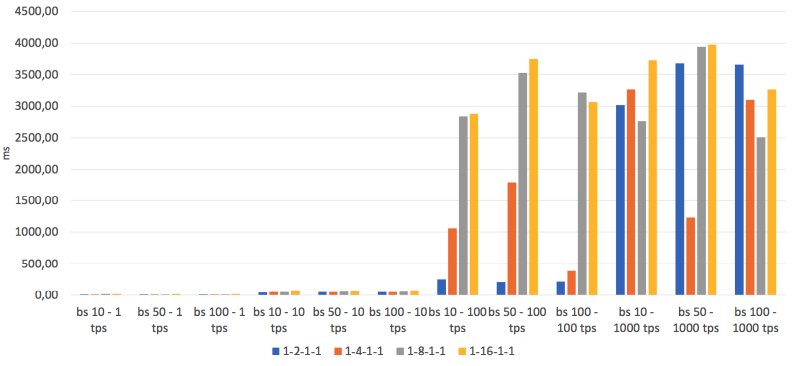
\includegraphics[width=0.6\linewidth]{Graphics/EscalaParesUnaOrganizacion.png}
\caption{Tiempo de ejecuci\'on en una orgnizaci\'on para diferente n\'umero de nodos pares.}
\label{EscalaParesUnaOrganizacion}
\end{figure}

Al aumentar el n\'umero de nodos pares dentro de una organizaci\'on, el tiempo de ejecuci\'on de la transacci\'on aumenta significativamente. Con tasas de \emph{TPS} por encima de 100, la diferencia entre la configuraci\'on m\'as baja que contiene dos pares y las configuraciones m\'as altas con 16 pares es tan grande como $3535ms$ en el escenario \emph{bs50-100tps}. Este comportamiento es esperado producto a una mayor comunicaci\'on y sobrecarga de sincronizaci\'on dentro de la red. Al analizar el mismo escenario con dos organizaciones, la tendencia general en lo que respecta al impacto en el rendimiento contin\'ua. La figura \ref{EscalaParesDosOrganizaciones} muestra resultados similares a la figura \ref{EscalaParesUnaOrganizacion}, pero ahora incluye dos organizaciones. Todos los pares se distribuyen por igual entre todas las organizaciones.\\

\begin{figure}[h]
\centering
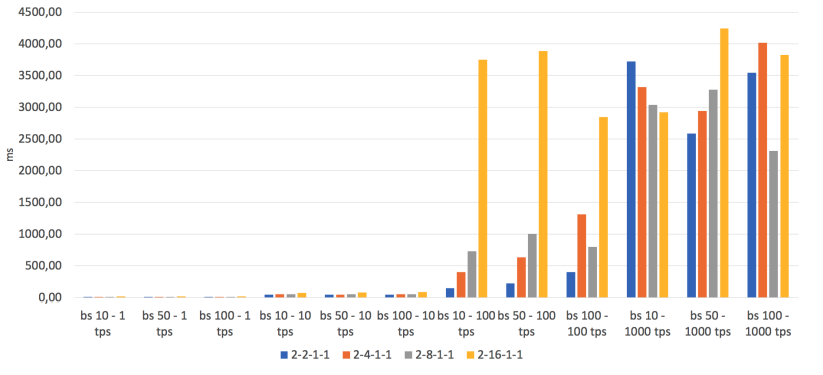
\includegraphics[width=0.6\linewidth]{Graphics/EscalaParesDosOrganizaciones.png}
\caption{Tiempo de ejecuci\'on en dos orgnizaci\'on para diferente n\'umero de nodos pares.}
\label{EscalaParesDosOrganizaciones}
\end{figure}

